\section{Η πορεία των πρωτονίων}
	Όπως έχει αναφερθεί, πέρα από τις συγκρούσεις βαρέων ιόντων, το πρόγραμμα του RHIC και των αντίστοιχων ανιχνευτών του περιλαμβάνει και συγκρούσεις πρωτονίων αλλά και πολωμένων πρωτονίων έως και ενέργειες $\sqrt{s} = 500GeV$.
	Κύριοι στόχοι εδώ είναι να μελετηθεί η προέλευση του σπιν των νουκλεονίων, καθώς εκτιμάται ότι τα κουάρκ συνεισφέρουν σε αυτό μόλις κατά ~25\% και επίσης να μελετηθούν ασυμμετρίες στις ενεργές διατομές διαφόρων δεσμών ανάλογα με την πόλωσή τους.
	
	Η δέσμη πολωμένων πρωτονίων ξεκινάει από μία πηγή πολωμένων ιόντων $H^-$.  Η πηγή μπορεί να παράξει ρεύμα 500$\mu A$ σε έναν παλμό διάρκειας $300\mu s$ ο οποίος περιέχει $9\times 10^{11}$ πολωμένα ιόντα $H^-$ σε ποσοστρό 80-85\% καθώς η εν λόγω παραγωγή αποτελείται από πολλά στάδια και σε κάθε ένα από αυτά χάνεται ένα μέρος της πόλωσης. Η τελική ενέργεια είναι 35keV ανά ιόν.
	
	Κατά την έξοδο από την πηγή, τα ιόντα εισέχονται στον γραμμικό επιταχυντή RFQ (Radiofrequenct Quadtrupole), ο οποίος τα επιταχύνει σε ενέργεια 753keV και τα οδηγεί στον LINAC. 
	Ο lINAC πρόκειται για ένα γραμμικό επιταχυντή αποτελεούμενο από κοιλότητες RF και που επιταχύνει τα ιόντα σε ενέργειες 200MeV. Στο τέλος της επιτάχυνσης από τον LINAC, η δέσμη περνάει από μία διαδικασία στην οποία απομακρύνονυαι τα δύο ηλεκτρόνια από το κάθε ιόν και απομένουν τα πολωμένα πρωτόνια που θέλουμε να μελετήσουμε και εν τέλει εισάγονται στον AGS Booster μειωμένα στον μισό πληθυσμό $4\times10^{11}$ ανά παλμό.
	Στον AGS-Booster επιταχύνονται στα 2.4GeV και έπειτα εισάγονται στον AGS ο οποίος τα επιταχύνει στα $24.3GeV$ και τότε οδηγούνται μέσω μίας γραμμής μεταφοράς στον RHIC. 
	Το σημαντικότερο στοιχείο στις επιταχύνσεις πρωτονίων είναι η δημιουργία και η διατήρηση της πόλωσής τους. Για να επιτευγχθεί αυτό χρησιμοποιούνται κάποιοι εξειδεικευμένοι μαγνήτες, οι Siberian Snakes.
	
	
 	Η επιτάχυνση πολωμένων πρωτονίων απαιτεί τον έλεγχο τόσο στην τροχιακή κίνηση, όσο και στην κίνηση του σπιν τους. Ο έλεγχος της τροχιακής τους κίνησης είναι παρόμοιος με αυτόν για τα βαρέα ιόντα, όμως ο έλεγχος του σπιν διαφέρει.
 	
 	
	Η δυναμική του σπιν των πρωτονίων δίνεται από την εξίσωση 
		\begin{align*}\label{eq2.8}
			\odv{\bm{S}}{t} = - \frac{e}{\gamma m}\left( G\gamma \bm{B}_\perp  + (1+G)\bm{B}_\parallel\right) \times\bm{S} \numberthis
		\end{align*}
	
	όπου $\bm{S}$ είναι το διάνυσμα του σπιν σε ένα σύστημα αναφοράς που κινείται μαζί με το σωματίδιο, $\bm{B}_\perp$, $\bm{B}_\parallel$ είναι οι συνιστώσες του μαγνητικού πεδίου κάθετα και παράλληλα στην κατεύθυνση της δέσμης, γ ο παράγοντας Lorentz και G η ανώμαλη μαγνητική ροπή, που για το πρωτόνιο ισούται με $G=1.7928$.
	
	Η σχέση (\ref{eq2.8}), άν δεν περιείχε τον πρώτο όρο, μοίάζει με την εξίσωση για σχετικιστική κίνηση φορτισμένου σωματιδίου σε εξωτερικό μαγνητικό πεδίο 
		\begin{align*}\label{eq2.9}
			\odv{\bm{u}}{t} = - \frac{e}{\gamma m} \bm{B}_\perp \times\bm{u} \numberthis
		\end{align*}
		
Παρατηρούμε πως στην ιδανική περίπτση που το πεδίο είναι μόνο κάθετο στην δέσμη, δηλαδή $\bm{B_\parallel}  = 0$, οι παραπάνω εξισώσεις διαφέρουν μονάχα κατά έναν παράγοντα $G\gamma$. Από αυτά μπορούμε να συμπαιρνάνουμε πως στην ιδανική περίπτωση η μεταπτωτική κίνηση του σπιν γίνεται $G\gamma $ φορές γρηγορότερα από την περιστροφική κίνηση του πρωτονίου.		
	Αυτή την διαφορά στις συχνότητες περιστροφής, την ποσοτικοποιούμε εισάγοντας μία νέα παράμετρο , το \textit{spin tune, }$v_{sp}$. Αυτή είναι μία παράμετρος η οποία ορίζεται ως ο αριθμός των περιστροφών της μεταπτωτικής κίνησης του σπιν σε μία πλήρη κυκλική περιστροφή του σωματιδίου. Στην ιδανική περίπτωση ισχύει ότι $v_{sp}=G\gamma$.\footnote{Στην υψηλότερη ενέργεια του RHIC, $\sqrt{s}=250GeV$ η τιμή της είναι $v_{sp}=476$}	
			
	Η δυσκολία στην επιτάχυνση πολωμένων δεσμών 	έγκειται στους  παράγοντες οι οποίοι καταστρέφουν την πόλωσή τους.
	Ενδεικτικά, ενδέχεται να υπάρχουν μικρά οριζόντια πεδία. Αυτά προκαλούν διαταραχές στο διάνυσμα του σπιν οι οποίες εν τέλει τείνουν να αθροίζονται και να απο-πολώνουν κάποια σωματίδια.
	Ακόμη, υπάρχει και ένας άλλος συντονισμός ο οποίος επιδεινώνει την πόλωση και  εμφανίζεται όταν $v_{sp}=v_{bet}$, όπου $v_{bet}$ το \textit{betatron tune}, δηλαδή ο αριθμός των ταλαντώσεων betatron σε μία πλήρη περιστροφή.
	
%	Για να ποσοτικοποιήσουμε την επίδοση στην διατήρηση της πόλωσης εισάγουμε μία νέα παράμετρο, το \textit{spin tune, }$v_{sp}$. Αυτή είναι μία παράμετρος η οποία ορίζεται ως ο αριθμός των περιστροφών της μεταπτωτικής κίνησης του σπιν σε μία πλήρη κυκλική περιστροφή του σωματιδίου. Στην ιδανική περίπτωση ισχύει ότι $v_{sp}=G\gamma$.
%	Η επιτάχυνση τέτοιων δεσμών γίνεται δύσκολη καθώς υπάρχουν διάφοροι παράγονται οι οποίοι καταστρέφουν την πόλωση. Για παράδειγμα
	
	
	\begin{figure}[h!]
		\centering
		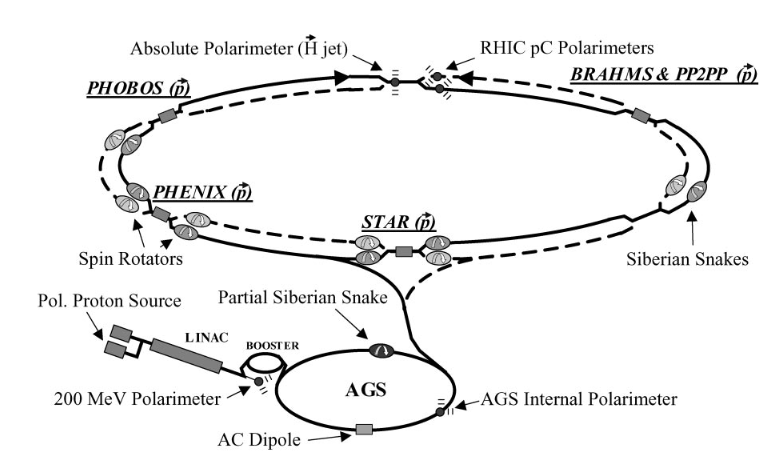
\includegraphics[scale=0.7]{Accelerating_System/protons_path}
		\caption{Η πορεία των πολωμένων πρωτονίων}
		\label{fig2.9}
	\end{figure}
	
	 Για παράδειγμα όταν η συχνότητα της μεταπτωτικής κίνσης του σπιν ισούται με την συχνότητα των μαγνητικών πεδίων που αλληλεπιδρούν με το σπιν, τότε προκαλείται ένας συντονισμός που μειώνει το ποσοστό των πολωμένων πρωτονίων της δέσμης.
 	Γενικότερα, οι κύριοι συντονισμοί που καταστρέφουν την πόλωση οφείλονται σε ατέλειες των μαγνητικών πεδίων και σε συντονισμούς οι οποίοι είναι εγγενείς στην αλληλεπίδραση σπιν-μαγνητικού πεδίου.
	Για παράδειγμα, αν υπάρχει μία ατέλεια του πεδίου η οποία διαταράσσει ελάχιστα το σπιν ενός διερχόμενου πρωτονίου περιστρέφοντάς προς τον άξονα της δέσμης, τότε κάθε φορά που ένας "παλμός" της δέσμης θα περνάει από εκείνο το σημείο της ατέλειας όλο και μεγαλύτερο ποσοστό των πολωμένων πρωτονίων θα χάσουν την πόλωσή τους. Αυτό το φαινόμενο καλείται \textit{συντονισμός αποπόλωσης} και εμφανίζεται σε ακέραιες τιμές του \textit{spin tune}, $v_{sp} = G\gamma =n, n\in\mathbb{N}$ 
 	%Ο δεύτερος συμβαίνει όταν $v_{sp} = G\gamma = 3k\pm v_y, k\in\mathbb{N}$ και $v_y$ είναι το εγκάρσιο \textit{betatron tune}.
 	
 
 
% 	Όταν η δέσμη περνάει μία περιοχή συντονισμού, τότε η τελική πόλωση $P_f$ σε σύγκριση με την αρχική $P_I$ δίνεται από την σχέση 
% 	\begin{align*}\label{eq2.8}
% 		\frac{P_f}{P_i} = 2 e^{-\frac{\pi r^2}{2\alpha}} - 1 \numberthis
% 	\end{align*}
%	
%	όπου α είναι η αλλαγή του \textit{spin tune} ανά ακτίνιο της τροχιάς και r είναι η ισχύς του συντονισμού. 
%	

%	Η αρχική πηγή πολωμένων πρωτονίων, παρέχει περίπου $10^12$ τέτοια σωματίδια σε κάθε παλμό ο οποίος εν συνεχεία επιταχύνεται στον AGS όπου μειώνονται τα πολωμένα πρωτόνια, καταλήγουν 2x$10^11$ στον RHIC.
%	Η πόλωση της δέσμης αλλάζει πρόσημο κάθε φορά που ικανοποιείται η συνθήκη συντονισμού $G\gamma = n, n\in\mathbb{N}$ και εν τέλει καταλήγουν στον RHIC 120 "παλμοί" από 2x$10^{11}$ πολωμένα πρωτόνια και με την \textit{emittance} της δέσμης λιγότερο από $20\mu m$.
		
	\begin{figure}[h!]
			\centering
			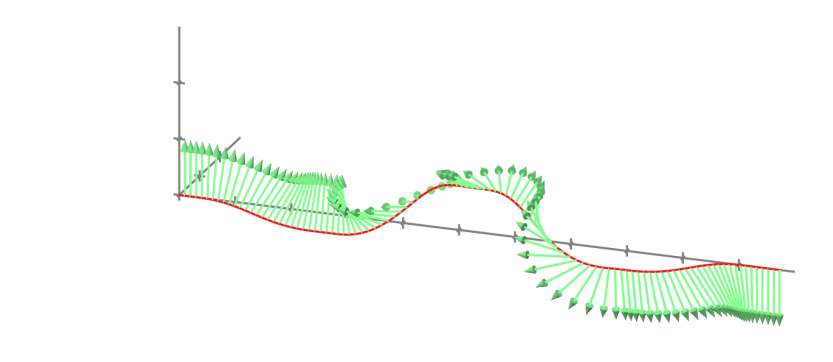
\includegraphics[scale=0.7]{Accelerating_System/traj_through_siberian}
			\caption{Η εξέλιξη της πόλωσης του spin κατά την διέλευση από έναν Siberian Snake μαγνήτη}
			\label{fig2.10}
		\end{figure}
		
	Στον RHIC, χρησιμοποιούνται οι μαγνήτες \textit{Siberian Snake} προκειμένου να διατηρήσουν την πόλωση της δέσμης.
	Αυτοί, προκαλούν συνολική περιστροφή της πόλωσης κατά 180$^o$ προς τον οάξονα της δέσμης, χωρίς να προκαλούν κάποια αλλοίωση στην τροχιά της δέσμης στο τέλος της διαδικασίας.
	Σε κάθε δαχτυλίδι του RHIC υπάρχουν 2 Siberian Snakes σε αντιδιαμετρικά σημεία, όπου ο καθένας αποτελείται από 4 υπεραγώγιμους ελικοειδής διπολικούς μαγνήτες μαγνητικού πεδίου εως 4Τ και μήκους 2.4m.

		
		
	Ακόμη, υπάρχουν 4 \textit{rotators}, οι οποίοι είναι μαγνήτες τοποθετημένοι σε κάθε δαχτυλίδι στις δύο άκρες του STAR (και άλλοι 4 για το PHENIX).
	Ο κάθε ένας τους αποτελείται από 4 διαδοχικά ελικοειδή δίπολα των οποίων τα πεδία ξεκινούν από κατακόρυφα και καταλήγουν διαμήκη. Έτσι κατά την είσοδο της δέσμης στην περιοχή αλληλεπίδρασης, υπάρχει η δυνατότητα να αλλάξουν την πόλωση από εγκάρσια σε διαμήκη ανάλογα με τις ανάγκες του πειράματος που δημιουργείται και κατά την έξοδό της να γίνει επαναφορά στην αρχική εγκάρσια πόλωση η οποία απαιτείται για την κίνηση εντός του RHIC.
	
	Οι διαφορετικές πολώσεις των πρωτονίων απαιτούνται για την μελέτη ασυμμετριών στις ενεργές διατομές. Για παράδειγμα, όπως θα δούμε στην συνέχεια, έχει βρεθεί διαφορά στις ενεργές διατομές συγκρούσεων προτονίων προς $\pi^0$ ανάλογα με το αν η πόλωση του σπιν των αρχικών πρωτονίων είναι κατακόρυφη προς τα πάνω ή προς τα κάτω.
	
	
		